\section{Introduction}

Midsurface is an abstracted representation of a thin-walled solid, used mainly for creating shell elements in the CAE meshing process. It can also be used as a shape-signature in shape matching/retrieval. It is expected to express the contiguous flow of the solid's shape  \cite{Rezayat1996}. So, to be truly effective, the midsurface needs to mimic the original solid, in both, geometrical and topological sense. Geometrically, the shape of the midsurface should be such that it lies in the middle (at half the thickness) of the solid. Topologically, the connectivity between the midsurface patches should be similar to that of their corresponding sub-shapes in the original solid. 

There are a large number of methods to compute the midsurface. They work on different input types of the original solid, such as, faceted mesh, Boundary Representation (Brep) solids, feature-based CAD models, etc. Quality of the output midsurface depends on the shape-characteristics of the original thin-walled solid.

\subsection{Thin-walled Solids}
Many thin-walled solids are from the sheet metal domain. These are unique in both, geometrical and topological sense. They are characterized by:
\begin{itemize}[noitemsep,topsep=2pt,parsep=2pt,partopsep=2pt,leftmargin=*]
\item \textbf{Constant thickness}: Sheet metal parts are made up of constant thickness blank roll.
\item \textbf{Absences}: There are no blind holes but only through holes, if any. 
\item \textbf{Degeneracy}: There are no degenerate capping thickness faces (like ``Wedge'').
\item \textbf{Cavities}: There are no embedded volumes or cavities (``bubbles'').
\end{itemize}

Quality of the output midsurface depends on the complexity of the original solid. The topological validation method for the midsurface developed in this work has been devised for solids exhibiting sheet metal shape characteristics. Such thin-walled solids, with constant thickness, pose lesser problems in the computation of the midsurface as well as in the validation of the midsurface, than the ones with variable thicknesses. Although the validation method mentioned in this work is derived for constant thickness solids, it can be extended to thin-walled parts with variable thickness as well, e.g., injection-molded plastic parts having drafts. Shape with or without draft angle are topologically the same, so the formulation developed in this work applies equivalently.

Many of the commercial sheet metal CAD modelers represent the thin-walled shape using a data-structure called Boundary Representation (Brep). Section 2 provides the characteristics of Brep and its classification into manifold and non-manifold representations. In this work, the term 'manifold' refers to an object which is bound, closed and homeomorphic to a topological sphere (also known as 2-manifold), whereas 'non-manifold' object does not have such restrictions of closure and completeness. This work uses 'non-manifold' mainly for surfaces, unless stated otherwise.


\subsection{Midsurface Computation}

Midsurface computation has been a widely-researched topic and there are many methods such as Medial Axis Transform, Chordal Axis Transform, and Midsurface Abstraction, etc.  \cite{Thakur2009}. Out of these, very few are based on the explicit shape transformation operators. 

Sheen et. al \cite{Sheen2008} used the deflation process to compute midsurface from a solid. Their algorithm did not change the topology but just reduced the capping entities to zero size. The problem with such an approach could be that the degenerated topology would be potentially detrimental to the downstream modeling operations.

Lee \cite{Lee2009a} proposed topological operators to transform a sheet of solid topology into a thin-walled solid by face geometry replacement. However, this method could pose difficulty in representing the adjacency relationships.

Even after extensive research in the academic domain and wide availability in commercial implementations, midsurface quality is still a concern. It suffers from errors like gaps, overlaps, missing surfaces, etc. Validating the output midsurface is a critical step in assessing the quality, after which corrective actions can be taken.

\subsection{Midsurface Validation}

To verify the quality of the midsurface, the following methods are used:

\begin{itemize}
[noitemsep,topsep=2pt,parsep=2pt,partopsep=2pt]
\item \textbf{Manual}: Manual inspection for errors such as missing surfaces, connection gaps, overlaps, etc. One needs to ensure that the midsurface lies midway and is continuous throughout, especially at the connections and steps. This method is obviously tedious, time-consuming and error-prone.
\item \textbf{Inspection Tools}: Tools provided in the CAD-CAE packages can detect gaps and overlaps but they can not detect the correctness of the midsurface at critical locations, such as connections and steps, where expectations could be  subjective.
\item \textbf{Geometric Tools}: Hausdorff distance from the midsurface to its original solid is computed. Accuracy of such methods depend on the sampling as well as on the complexity of the surface representation, making them computationally intensive and error-prone. 
\item \textbf{Topological Validation}: This involves comparison of the number of predicated topological entities with the actual ones, and if there is a mismatch, the  problem is detected. Here, the geometry of the shape, is ignored. It has an advantage over geometric validation since computationally intensive distance calculations are not performed. 
\end{itemize}

This work proposes a novel method for the topological validation of midsurface of thin-walled solids.

\subsection{Topological Validation}  
Topological validation proposed in this work proposes two transformations with which the quality of a midsurface can be assessed. First, solid-to-surface, where, the dimension-reduction transformation equations are applied to the thin-walled solid to predict the topological entities of the corresponding midsurface and then compared with the actual topological entities of the output midsurface. In the second approach, surface-to-solid, dimension-addition transformation equations are applied to the output midsurface to predict the topological entities of the corresponding thin-walled solid, and then compared with the actual topological entities of the thin-walled solid.

The validation method presented in this work cannot be used in isolation from geometry. As the midsurface is applicable only for the thin-walled solids, it is not computed and validated using this method for thick solids. But such differentiation of the solid-shape, being thick or thin, is 'geometrical' and not 'topological', which this method itself cannot detect. So, the work presented below should be used only for the known thin-walled solids for which midsurface are computable.

Use of topology for assessing the quality of midsurface is not widespread and there are very few such attempts reported in the literature.


Lipson \cite{Lipson} stated that a topological invariant for all the sheet metal parts and thin-walled objects can be used as a necessary condition for topological validity and reasoning .  

Lockett and Guenov \cite{Lockett2008} used both geometric and topological variants for checking the validity of the midsurface. For geometric validation, they used the Hausdorff distance between a midsurface and its corresponding principal faces (pairs). For topological validation, they used proximity groups adjusted by an angle criterion. The main limitation of their approach appears that the geometric criteria (closest distance proximity or angle between faces) are used in the topological validations, which, ideally, should not be the case.

Apart from CAE, skeletal structures such as midsurface are used in CAD model comparison solutions such as shape-based retrieval, similarity assessment and difference identification  \cite{Antoine2014}. Skeletal graph matching is one of the prominent techniques \cite{Iyer2005} for similarity assessment. A topologically valid midsurface represents sub-shape connectivities better and thus acts as more effective shape-signature in the model comparison.

The work presented here, provides with transformation relations and a topological variant, based purely on the combinatorial topology for determining the validity of a midsurface computed from a sheet metal part.

\section{Preliminaries}\label{sec_preliminaries}
\subsection{Boundary Representation (Brep)}

Brep is composed of two parts: topology and geometry. Topological elements are shells, faces, edges, vertices, etc. They are mentioned in the descending order of the topological dimensionality:

\begin{itemize}
[noitemsep,topsep=2pt,parsep=2pt,partopsep=2pt]
\item {\em shell (s)}  is a connected set of {\em faces}
\item {\em face (f)} is a bounded portion of a {\em surface} (geometry)
\item {\em loop (l)} is a circuit of {\em edges} bounding a {\em face}
\item {\em half-edges (he)} are used to create a {\em loop}.
\item {\em edge (e)} is a bounded portion of a {\em curve} (geometry)
\item {\em vertex (v)} lies at a {\em point} (geometry). 
\end{itemize}

Validity of the Brep model is checked using the Euler-Poincar\'e equation.

\subsubsection{Euler-Poincar\'e Equation}
Euler's equation for polyhedral solids is: $$v - e + f = 2$$ where, $v$, $e$, and $f$ represent the number of vertices, edges and faces respectively. It was discovered by Leonhard Euler in 1752 and was later generalized by Lhuilier \cite{Krishnamurti2002} as follows: $$v - e + f = 2 - 2g$$ where, $g$ represents genus, the number of holes $h$ or handles ($g$ and $h$ are considered interchangeable in this paper). Later on, Schläfli and Poincar\'e also generalized the formula to the higher dimensional n-polytopes. 

The Euler characteristic ($\chi$) for combinatorial cell complexes or polyhedral solids is defined as below:

\begin{equation}
\sum_{i=0 }^D(-1)^{i} N_{i}= \sum_{i=0}^D(-1)^{i} \beta_{i} = \chi 
\label{eqn_betti}
\end{equation}
For dimensions upto 3 ($i=3$), equation (\ref{eqn_betti}) simplifies to:
\begin{equation}
N_{0}-N_{1}+N_{2}= \beta_{0} -\beta_{1} + \beta_{2}
\label{eqn_betti3}
\end{equation}

where, $N$s are topological entities of the dimension $0,1$ and $2$ respectively and $\beta$s are the Betti numbers. $\beta_{0}$, $\beta_{1}$ and $\beta_{2}$ correspond to  the number of connected components, holes and cavities, respectively \cite{Sequin}. 

Two homeomorphic topological spaces will have the same Euler characteristic and Betti numbers.

Most of the CAD models are made up of solids (manifolds), since they are considered to be complete and  having their own volumes. A manifold-solid model  can only represent one closed volume minus its internal structure. It cannot represent  heterogeneous possibilities such as wires (curves),  sheets (surfaces),  and  solids (volumes) together, which although, are not possible in the real world, but are possible during the intermediate stages of design \cite{Yamaguchi1995}. A non-manifold model is a generic modeling framework which encompasses all these items in a single framework \cite{Lee2001}.

The Euler characteristic ($\chi$) in terms of Betti numbers, provides a generic invariant for a shape of any dimension. Manifestation of the Betti numbers in different dimensions is different. So, when a thin-walled solid is transformed into its corresponding midsurface, the interpretation of the Betti numbers changes from the manifold domain to the non-manifold domain.

\subsubsection{Manifold-Solids}
The Euler Poincar\'e equation for manifold-solids is:
%\vspace{-2mm}
\begin{equation}
v - e + (f - r) = 2 (s - h)
\label{eqn_manifold}
\end{equation}

Its equivalence with equation (\ref{eqn_betti3}) is as follows:

\begin{itemize}
[noitemsep,topsep=2pt,parsep=2pt,partopsep=2pt,label={}]
\item $N_{0} = v $ : number of vertices
\item $N_{1} = e $ : number of edges
\item $N_{2} = (f - r)$ : number of faces ($f$) - additional {\em artifact} edges corresponding to inner loops ($r$)
\item $\beta_{0} = s$ : number of components or disjoint parts ($shells$)
\item $\beta_{1} = 2h$ : number of independent closed curves drawn without splitting. Twice the genus $g$ or $h$. For Torus, there are two such circles and one genus-hole. ($2h$)
\item $\beta_{2} = s$ : number of space regions created by connected surfaces. For an open surface $\beta_{0} = 1$ and $\beta_{2}=0$ whereas for closed surface,  $\beta_{2}$ is equal to $\beta_{0}$,  which is equal to $s$.
\end{itemize}

\subsubsection{Non-manifold-Surfaces}
Solids found in the real world have the property that on any point on the boundary, a small enough sphere at that location is split into two pieces, one inside and one outside the object. Non-manifolds do not obey this rule \cite{Krishnamurti2002}. Weiler (\cite{Weiler1986}) can be attributed for the first significant contribution in defining the non-manifold data structure, called {\em Radial Edge Structure}. Core to this data structure lies the radial cycle, which is an ordered list of faces around an edge. Similar to manifold, equation for non-manifold topology \cite{Yamaguchi2002} is: 

\begin{equation}
v - e + (f - r) = s - h
\label{eqn_nonmanifold}
\end{equation}

Its equivalence with equation (\ref{eqn_betti3}) is as follows:

\begin{itemize}
[noitemsep,topsep=2pt,parsep=2pt,partopsep=2pt,label={}]
\item $N_{0} = v$ : number of vertices
\item $N_{1} = e$ : number of edges
\item $N_{2} = (f - r)$ : number of faces ($f$) -  inner loops ($r$)
\item $\beta_{0} = s$ : number of components or disjoint parts ($shells$)
\item $\beta_{1} = h$ : number of independent closed curves drawn without splitting. Inner holes ( $g$ or $h$). 
\item $\beta_{2} = 0$ : number of space regions created by connected surfaces are not present; so it is $0$.
\end{itemize}

\subsection{Cellular Decomposition}
Cellular topology is one of the prominent representations in solid modeling.  The  fundamental unit is called $Cell$, which has dimensionality $0/1/2/3$ and can have adjacency to its neighbor denoted as $Cell_{dimension,adjacency}$. Actual size and the shape of the cells can vary based on the underlying geometry (Table \ref{tbl_celldecompexample}). 


\begin{minipage}{0.9\linewidth}
%\begin{minipage}{0.9\textwidth} %should be full length even in case of two column
%\resizebox{0.9\linewidth}{!}{
\begin{center}
\begin{tabular}[h]{@{}p{0.22\linewidth} p{0.22\linewidth}  | p{0.22\linewidth}  p{0.22\linewidth} @{}} \toprule
{\bf Original Part} & {\bf Cellular Model}  & {\bf Original Part} & {\bf Cellular Model} \\ \midrule  

\adjustbox{valign=t}{\includegraphics[width=0.8\linewidth]{../Common/images/nonCellularL}}  &  
\adjustbox{valign=t}{\includegraphics[width=0.8\linewidth]{../Common/images/CellularL}}  &

\adjustbox{valign=t}{\includegraphics[width=0.8\linewidth]{../Common/images/nonCellularT}}  &  
\adjustbox{valign=t}{\includegraphics[width=0.8\linewidth]{../Common/images/CellularT}} 
\\ \midrule

\adjustbox{valign=t}{\includegraphics[width=0.8\linewidth]{../Common/images/nonCellularOverlap}}  &  
\adjustbox{valign=t}{\includegraphics[width=0.8\linewidth]{../Common/images/CellularOverlap}}  &

\adjustbox{valign=t}{\includegraphics[width=0.8\linewidth]{../Common/images/nonCellularZU}}  &  
\adjustbox{valign=t}{\includegraphics[width=0.8\linewidth]{../Common/images/CellularZU}} 
\\ %\midrule

\bottomrule
\end{tabular}
\captionof{table}{Decomposition of shapes into Cells}
\label{tbl_celldecompexample}
\end{center}
%}
\end{minipage}


\subsubsection{Cellular Entities}
Cellular Decomposition is a process by which a shape (called ``Original solid'') is split in to multiple sub-shapes (called ``Cells'').   According to Chen et al. \cite{Chen2006}, a cellular model includes topologies of various dimensions. 
$$\mathbb{M} = 
(\cup_{i=1}^{q} C_i^0 ) \cup 
(\cup_{j=1}^{r} C_j^1 ) \cup  
(\cup_{k=1}^{s} C_k^2 ) \cup 
(\cup_{l=1}^{t} C_l^3 ) $$ where  $C_i^0$ are $0$-dimensional vertices,  $C_j^1$ are $1$-dimensional edges,  $C_k^2$ are $2$-dimensional faces and  $C_l^3$ are $3$-dimensional solids. The cells have the following properties: 
	\begin{itemize}[noitemsep,topsep=2pt,parsep=2pt,partopsep=2pt]
	\item \textbf{Boundary}: Except $C_i^0$ cells, all cells are bound by cells with a dimension lower by 1.
	\item \textbf{Overlap}: No cells overlap.
	$C_i^a \cap C_j^b = \phi, ( 0 \leq a, b \leq 3, (a = b) \wedge ( i \neq j ))$
	\item \textbf{Nature}: Either  additive  or  subtractive.
	\end{itemize}

Cells can be of following types:

\begin{tabular}[h]{@{}p{0.1\linewidth} p{0.1\linewidth} p{0.4\linewidth} p{0.4\linewidth}@{}} \toprule

$Cell_{3,*}$  & 
\adjustbox{valign=t}{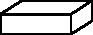
\includegraphics[width=\linewidth]{../Common/images/SimplePlate1.pdf}} &
3D cells (solids), topologically similar to a simple plate &
 $faces=6 \newline edges=12 \newline vertices =8$ \\
 
 $Cell_{2,*}$ &
 \adjustbox{valign=t}{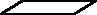
\includegraphics[width=\linewidth]{../Common/images/SimplePlane1.pdf}} &
  2D cells, topologically similar to a planar surface  &
   $faces=1 \newline edges=4 \newline vertices =4$ \\
   
$Cell_{1,*}$ &
 \adjustbox{valign=t}{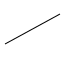
\includegraphics[width=\linewidth]{../Common/images/SimpleLine1.pdf}} &
1D cells, topologically equivalent to a line &
 $edges=1  \newline vertices =2$ \\
 
 $Cell_{3,h}$ &
  \adjustbox{valign=t}{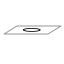
\includegraphics[width=\linewidth]{../Common/images/SimpleHole1.pdf}} &
  Hole is assumed to be cylindrical through-all (true for sheet metal parts) &
   $edges=1  \newline vertices =1$ \\ \bottomrule

 \end{tabular}

\subsubsection{Classification of Cells}
When the original solid is decomposed into distinguishable cells, new interface boundaries are introduced. Newly-created intersecting volumes or touching boundaries are called interface-cells, which can be either 3D (solids) or 2D (faces) respectively. 

\begin{itemize}[noitemsep,topsep=2pt,parsep=2pt,partopsep=2pt]
\item Two shapes touching each other with an area-overlap, is called 2d-Interface.
\item Two shapes touching each other with a volume-overlap, is called 3d-Interface.
\end{itemize}
	
If two bodies spatially overlap then they are split to form the 3D interface  (Fig. ~\ref{fig:3dinterface})  cell. In case of 2D Interface (Fig. ~\ref{fig:2dinterface}), adjoining faces of the overlapping face are extended \cite{Woo2002} and used as a  cutting tool to create the intersecting volume, the 3D Interface (Fig. ~\ref{fig:3dinterface}) cell.

%\begin{tabular}[htp]{@{} p{0.4\linewidth} p{0.05\linewidth}  p{0.4\linewidth}@{}} 
%
%\adjustbox{valign=t}{
\begin{minipage}[t]{\linewidth}
\centering 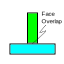
\includegraphics[width=0.4\linewidth]{..//Common/images/Interface2d_1.pdf}
%\caption{Caption1}
\captionof{figure}{2D Interface}
\label{fig:2dinterface}
\end{minipage}
%}
%
%&  &
%
%\adjustbox{valign=t}{
\begin{minipage}[t]{\linewidth}
\centering 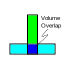
\includegraphics[width=0.4\linewidth]{..//Common/images/Interface3d_1.pdf}
%\caption{Caption1}
\captionof{figure}{3D Interface}
\label{fig:3dinterface}
\end{minipage}
%} \\
%
%\end{tabular}


\vspace{1mm}

%\begin{tabular}[htp]{@{} p{0.3\linewidth} p{0.05\linewidth}  p{0.55\linewidth}@{}} 
Prefix $s$ is applied if the $Cell$ is from the original solid, $i$ if it is of a newly-introduced interface type,(Fig.~\ref{fig_celldecompexample}) and $m$ for midsurface cells.

%&&

%\adjustbox{valign=t}{
\begin{minipage}[t]{\linewidth}
\centering 
\includegraphics[width=0.6\linewidth]{../Common/images/CellDecompExample}
%\vspace{\abovecaptionskip}
\captionof{figure}{Decomposition \& classification\cite{Treeck}}
\label{fig_celldecompexample}
\end{minipage}
%}		
%\\
%\end{tabular}

